\chapter{Literature Review}

There have been a lot of work in exploting zero-permission sensors found in a typical smartphone. Such security and privacy breaches via sensors have been investigated in publications like \cite{gyrophone}, \cite{walnut}, \cite{goespin}, \cite{spiphone}, \cite{accelprint} etc.

In \textbf{Gyrophone} \cite{gyrophone}, the authors showed how a Gyroscope could be used as a Microphone, but since they too were limited by the sampling rate, they used machine learning techniques (like SVM, GMM, DTW) to test their accuracies on Speaker, Gender Identification tasks. Speech Recognition was done on the TIDIDIGITS dataset. They also had a section where they used multiple such phones gathering data and then used it to further improve the accuracy of the model. Our goal with this project is to perform something similar with accelerometer data.

In the \textbf{Walnut} attack \cite{walnut}, the authors found critical vulnerabilities in the design of MEMS accelerometers, that could potentially allow an attacker to completely control the sensor readings being output. These sensors are not exclusively used on mobile phones, but in another devices as well, such as the SensorTile kit - which we discuss in a later section. The walnut attack requires frequencies close to the resonant frequency of the sensor (which need to be found out experimentally or from a datasheet by the manufacturer.) Essentially, this work further solidified the fact that that accelerometers (like gyroscopes) are susceptible to acoustic interferences in their vicinity.

As an example of an attack that is a bit different from acoustic injections, the authors of \cite{goespin} used a combination of zero permission sensors to guess a user’s PIN. This required modelling of the touch events and then some feature engineering and machine learning techniques (KNN, GNB, MLP, RF etc.) As their result they found that a combination of sensors (accelerometer + gyroscope) worked best.

\newpage

\section{Browsers}

Exploitation of these sensors on a modern smartphone doesn't always require creating a specialized application for the platform, as the authors of \cite{touchsig} showed, sensor data is also readily available via any modern browser - such as Firefox, Chrome etc. This has far reaching consequences, because this means that any website could capture sensor data and upload it to their server for later offline processing - coupled with existing web fingerprinting techniques - this could be used to target user behaviour and worst of all this raises absolutely no flags, or permission popups!

Since the paper came out, browser vendors have implemented further hardening techniques to make the exploit tougher, specifically, they have restricted the sampling rates and only web pages with secure contexts can capture data in background.

To understand this explot better, and confirm that the restrictions were in place, we created a demo webpage in Javascript that uses the window.ondevicemotion API to gather data (from motion sensors.)

Figure \ref{fig:brw_chrome} shows the Google Chrome browser, and the data frequency has been further reduced (from 200Hz to 60Hz.)

But, as Figure \ref{fig:brw_firefox} shows this is not the case with Firefox. It still allows sampling at a rate of 200Hz. So is still vulnerable to all sorts of sensor recording exploits.

\begin{figure}[H] \begin{center}
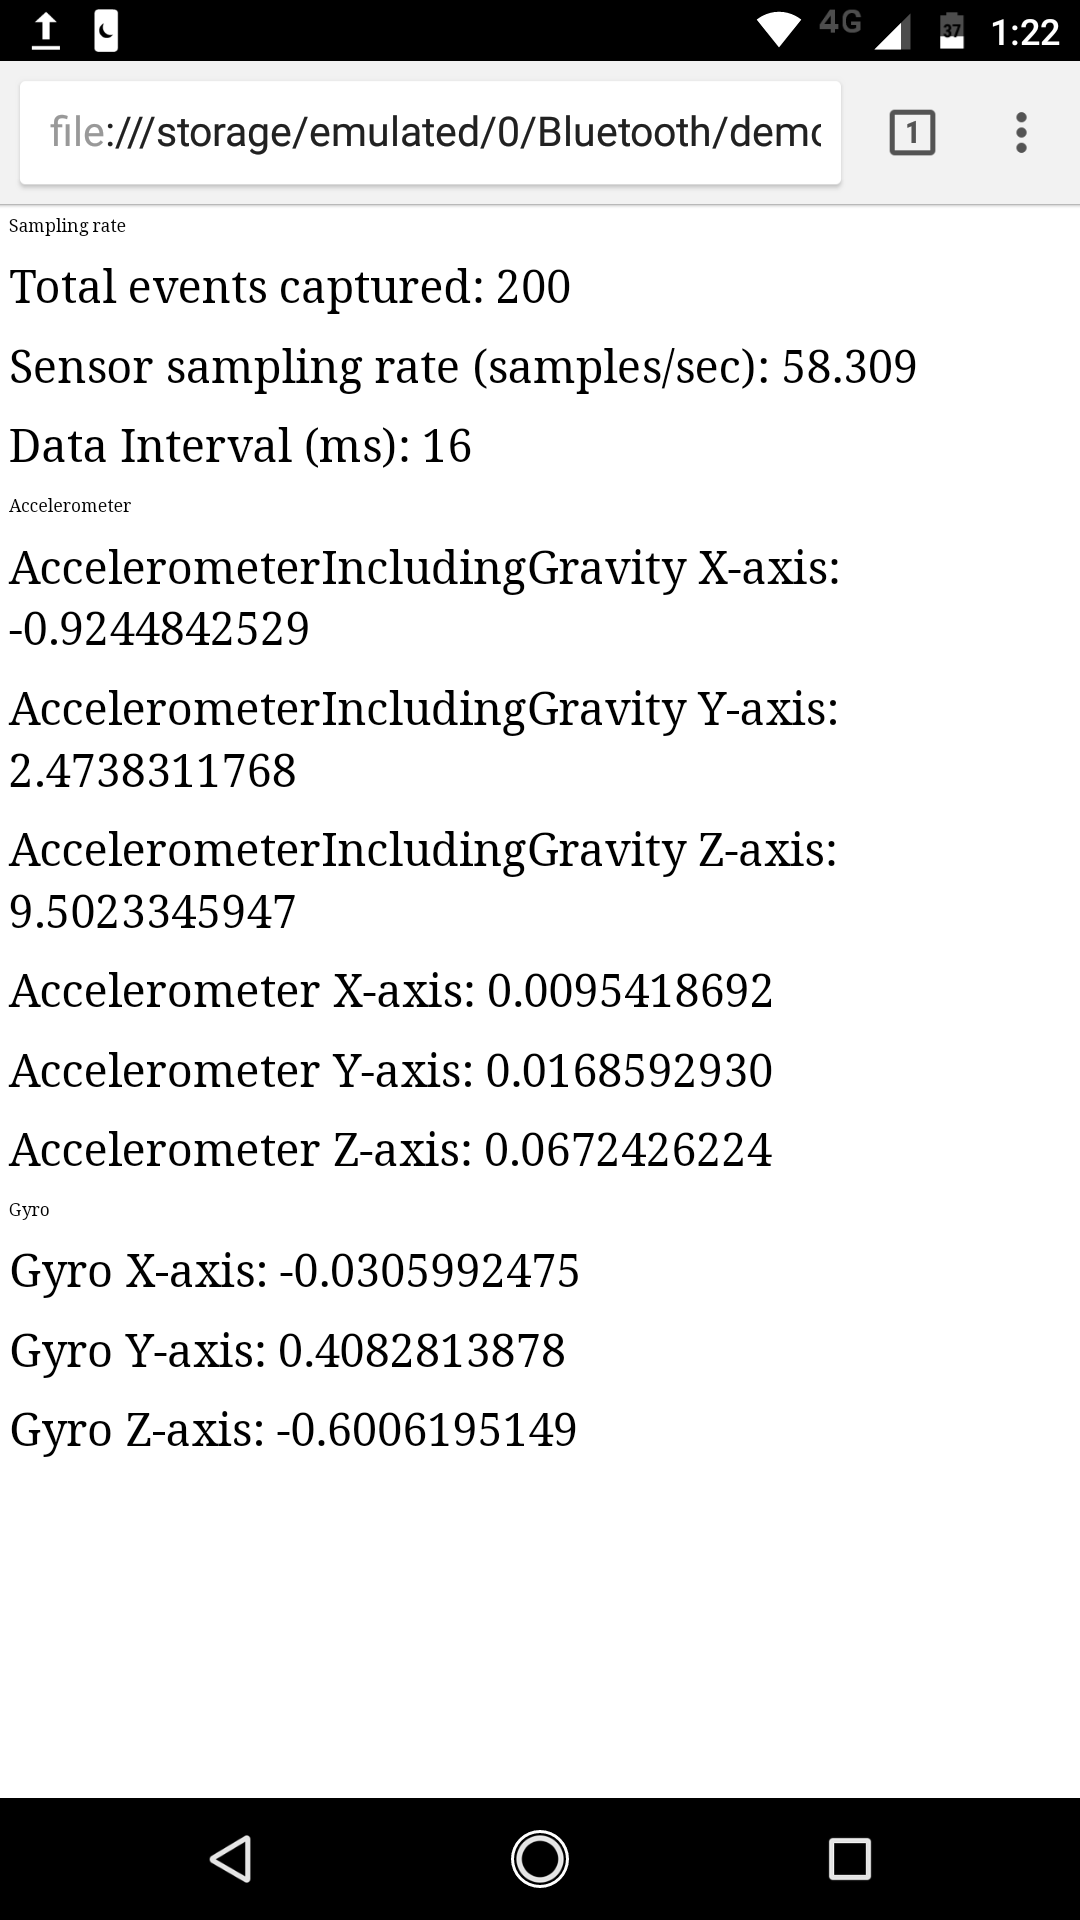
\includegraphics[scale=0.1]{brw_chrome}
\caption{A webpage recording motion sensors on Chrome (60Hz)}
\label{fig:brw_chrome}
\end{center} \end{figure}

\begin{figure}[H] \begin{center}
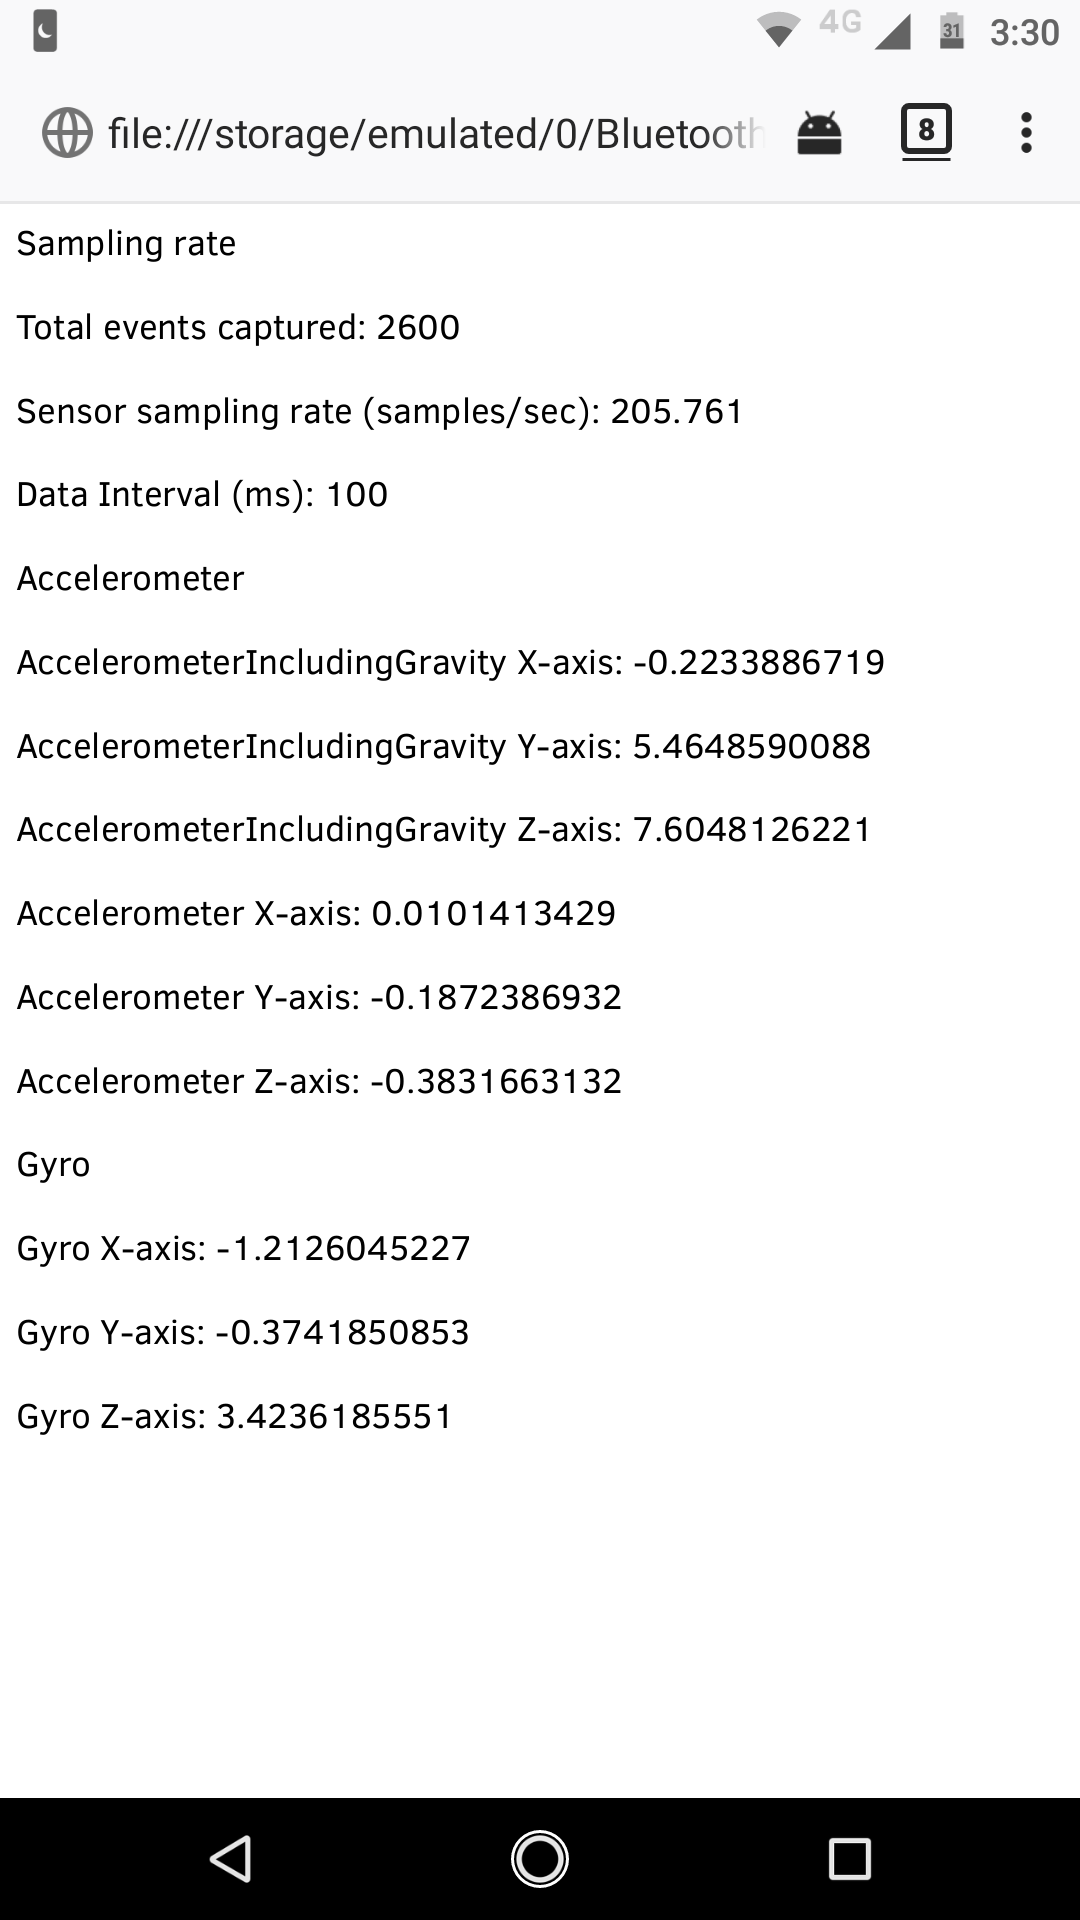
\includegraphics[scale=0.1]{brw_firefox}
\caption{A webpage recording motion sensors on Firefox (200Hz)}
\label{fig:brw_firefox}
\end{center} \end{figure}
